 \let\negmedspace\undefined
\let\negthickspace\undefined
\documentclass[journal]{IEEEtran}
\usepackage[a5paper, margin=10mm, onecolumn]{geometry}
%\usepackage{lmodern} % Ensure lmodern is loaded for pdflatex
\usepackage{tfrupee} % Include tfrupee package

\setlength{\headheight}{1cm} % Set the height of the header box
\setlength{\headsep}{0mm}     % Set the distance between the header box and the top of the text
\usepackage{gvv-book}
\usepackage{gvv}
\usepackage{cite}
\usepackage{amsmath,amssymb,amsfonts,amsthm}
\usepackage{algorithmic}
\usepackage{graphicx}
\usepackage{textcomp}
\usepackage{xcolor}
\usepackage{txfonts}
\usepackage{listings}
\usepackage{enumitem}
\usepackage{mathtools}
\usepackage{gensymb}
\usepackage{comment}
\usepackage[breaklinks=true]{hyperref}
\usepackage{tkz-euclide} 
\usepackage{listings}
% \usepackage{gvv}                                        
\def\inputGnumericTable{}                                 
\usepackage[latin1]{inputenc}                                
\usepackage{color}                                            
\usepackage{array}                                            
\usepackage{longtable}                                       
\usepackage{calc}                                             
\usepackage{multirow}                                         
\usepackage{hhline}                                           
\usepackage{ifthen}                                           
\usepackage{lscape}



\usepackage{amsmath,amssymb}
\usepackage{booktabs}
\usepackage{tikz}
\usetikzlibrary{arrows.meta,angles,quotes}





\begin{document}

\bibliographystyle{IEEEtran}
\vspace{3cm}

\title{4.12.28}
\author{AI25BTECH11023 - Pratik R}
% \maketitle
% \newpage
% \bigskip
{\let\newpage\relax\maketitle}

\renewcommand{\thefigure}{\theenumi}
\renewcommand{\thetable}{\theenumi}
\setlength{\intextsep}{10pt} % Space between text and floats


\numberwithin{equation}{enumi}
\numberwithin{figure}{enumi}
\renewcommand{\thetable}{\theenumi}


\section*{\textbf{Question}}
The value of the $\lambda$,  if the lines\\$(2x+3y+4)+\lambda(6x-y+12)=0$ are

\begin{tabular}[12pt]{ |c| c|}
    \hline
    \textbf{Points} & \textbf{Name}\\ 
    \hline
	\myvec{7\\10} & Point $\Vec{A}$ \\
    \hline 
	\myvec{-2\\5} & Point $\Vec{B}$\\
    \hline
	\myvec{3\\4} & Point $\Vec{C}$\\
    \hline
\end{tabular}

\subsection*{\textbf{Solution:}} 
Equation of line is given by
\begin{align}
    \myvec{2+6\lambda &3-\lambda} \vec{x} &=-4-12\lambda\\
    \implies \vec{n}^\top \vec{x} &= c;
\end{align}
where $\vec{n}^\top = \myvec{2+6\lambda &3-\lambda}$\\
and $c=-4-12\lambda$. \\
\begin{enumerate}

\item If the line is parallel to Y axis
\begin{align}
\vec{n}^\top \vec{e_2} &=0 \\
3 -\lambda &= 0 \\
\lambda &= 3
\end{align}




\item If the line is perpendicular to $7x+y-4=0$, that is, $\vec{n_1}^\top =\myvec{7&1}$
\begin{align}
    \vec{n_1}^\top \vec{n} &= 0 \\
    41\lambda &= -17 \\
    \lambda &= \frac{-17}{41}
\end{align}

\item If the line passes through $P(1,2)$
\begin{align}
  \vec{n}^\top \vec{P} &= c \\
  16\lambda &= -12 \\
  \lambda &= \frac{-3}{4}
\end{align}

\item If the line is parallel to X axis
\begin{align}
\vec{n}^\top \vec{e_1} &=0 \\
2+6\lambda &= 0 \\
\lambda &= \frac{-1}{3}
\end{align}
\end{enumerate}

\begin{figure}[H]
\centering
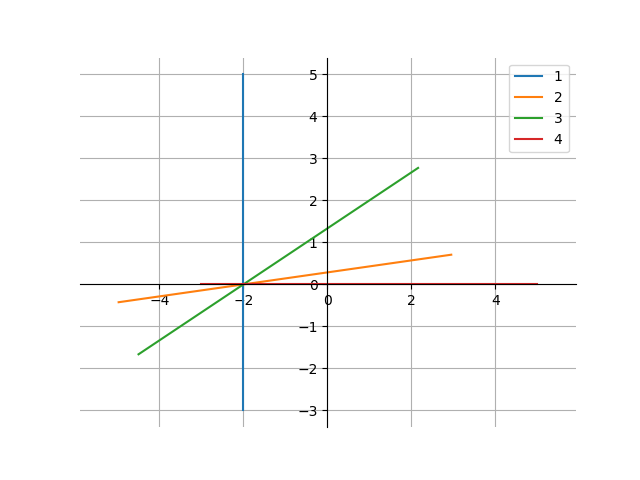
\includegraphics[width=0.7\columnwidth]{figs/fig.png} 
\caption{plane}
\label{}
\end{figure}

\end{document}
